\appendices

\section{Mechanism-solver construction}
\label{app:mechanism}

The mechanism solution $(\sigma, p_1,\dots,p_n)$ for a given action
profile $\boldsymbol{\eps}$ is obtained by a nested bisection. For
each candidate $\sigma$, we find the largest per-group $p_g$ that
satisfies the $I$-fold $(p_g, \sigma)$-subsampled Gaussian at
$(\eps_g, \delta)$-DP under \eqref{eq:budget}. Because the achieved $\eps$ is
monotone-increasing in $p_g$, a unique $p_g \in (0, 1]$ exists
(capped at $1$ if the budget cannot be exhausted); we locate it by
binary search using the \ac{RDP} accountant~\cite{mironov2017renyi}
until the achieved $\eps$ matches $\eps_g$ to a relative tolerance of
$10^{-3}$. We then bisect $\sigma$ on top of this inner search, using
the realised batch size $\hat B(\sigma) = \sum_g |G_g|\, p_g(\sigma,
\boldsymbol{\eps})$ as the outer-loop monitor, until $\hat B$ matches
$B$ to the same tolerance. Profiles in which any $p_g$ falls below
$10^{-5}$ are flagged infeasible per \cref{ass:participation}; below
that threshold the group's contribution to \eqref{eq:batch} is numerically
negligible and the \ac{iDP} contract is trivially satisfied. The
qualitative results are insensitive to this threshold across
$[10^{-6}, 10^{-3}]$ (\cref{app:sensitivity}).

Once $(\sigma, p_g)$ is fixed, the realised \ac{MIA} advantage of group
$g$ is computed exactly from the privacy-loss distribution of the
$I$-fold $(p_g, \sigma)$-subsampled
Gaussian~\cite{google-dp-accounting} by evaluating the trade-off
function and~\eqref{eq:adv}. This matches the formulation of
\citet{kaiser2026your} and yields the tightest analytical \ac{MIA}
advantage for the resulting mechanism.

\section{Proofs for \texorpdfstring{\cref{sec:analysis}}{Section IV}}
\label{app:proofs}

\subsection{Proof of \texorpdfstring{\cref{lem:externality}}{the externality lemma}}
\label{app:proof-externality}

We track how the solver absorbs one tightened budget. Everything rests
on two hypothesis-testing facts about a single $(p,\sigma)$
mechanism; the rest is bookkeeping through the two constraints.
\emph{(i) More sampling leaks strictly more:} for $p < p'$, the
member hypothesis at rate $p$ is a convex blend of the one at rate
$p'$ with the non-member hypothesis (with weight $1 - p/p'$ on the
null), and blending an alternative toward the null makes every test
strictly weaker. \emph{(ii) More noise leaks strictly less:} at fixed
$p$, the two hypotheses sit at mean shift $1/\sigma$, which shrinks
as $\sigma$ grows. Both orderings survive $I$-fold
composition~\cite{dong2022gaussian}; together they are amplification
by subsampling~\cite{balle2020privacy}. Hence the budget a mechanism
achieves at the shared $\delta$, $\eps(p, \sigma)$, is smooth,
strictly increasing in $p$, and strictly decreasing in $\sigma$.

Now solve the constraints in order. Constraint \eqref{eq:budget} inverts fact (i): at a
given $\sigma$, group $g$'s binding rate $p_g(\sigma, \eps_g)$ is
the unique rate whose leakage exhausts the budget, and it rises in
$\eps_g$ (a looser budget permits more sampling) and in $\sigma$
(more noise creates sampling room, by (ii)). Constraint \eqref{eq:batch} then pins
$\sigma$: the expected batch $F(\sigma) := \sum_g |G_g|\,
p_g(\sigma, \eps_g)$ is strictly increasing in $\sigma$, so exactly
one $\sigma$ delivers $B$.

Finally, tighten $\eps_j$. At the old $\sigma$ only $p_j$ moves,
downward, so the batch undershoots $B$; lowering $\sigma$ would
lower every rate and undershoot further, so the unique restoring
direction is $\sigma \uparrow$. Implicit differentiation of
$F(\sigma) = B$
makes this quantitative,
\[
\frac{\partial \sigma}{\partial \eps_j}
\;=\; -\,\frac{|G_j|\; \partial p_j / \partial \eps_j}{F'(\sigma)}
\;<\; 0 ,
\]
and every other group's budget is unchanged, so its rate moves only
through the noise: $\partial p_i / \partial \eps_j = (\partial p_i /
\partial \sigma)(\partial \sigma / \partial \eps_j) < 0$. Note where
the argument stops: if some $p_g$ caps at $1$ (a budget the noise
cannot exhaust), \eqref{eq:budget} stops binding for that group and the signs
can degenerate---the saturation corner excluded by the hypotheses
and met once in \cref{sec:experiments}. \qed

\subsection{Proof of \texorpdfstring{\cref{cor:externality-small-p}}{the small-p corollary}}

For a single step, the trade-off function of the subsampled pair is
\emph{exactly} the mixture $T_{p,\sigma}(\alpha) = (1-p)(1-\alpha) +
p\, T_\sigma(\alpha)$: the likelihood ratio of the mixture against
the base Gaussian is monotone in the same statistic as the
unsubsampled pair, so the same tests are optimal
(\cite{balle2020privacy}, Poisson-subsampling amplification). Its
sup-gap---the advantage, which equals the total-variation distance of
the pair---is therefore exactly $p\,\Adv_G(\sigma)$ per step, and
total variation is additive to leading order under $I$-fold products:
\begin{align*}
A(p,\sigma) &\;=\; I\, p\, \Adv_G(\sigma) + O\bigl((I p)^2\bigr),\\
\frac{\partial^2 A}{\partial p\, \partial \sigma}
    &\;=\; I\,\Adv_G'(\sigma) + O(I^2 p),
\end{align*}
the latter negative, valid in the regime $I p \ll 1$ (the composed
remainder is controlled by the product $Ip$, not by $p$ alone).
For the externality sign, substitute the small-$p$ closed
form $p_i = \sigma\sqrt{\rho_i}/\sqrt{2I\alpha}$ behind
\eqref{eq:sigma-implicit} into the chain rule for $\partial
\Apld{i}/\partial\eps_j$ and factor out
$(\partial\sigma/\partial\eps_j)<0$, which yields
\eqref{eq:proof-bracket}. The bracket is the $\sigma$-derivative of
$\sigma\,\Adv_G(\sigma)$ divided by $\sigma$; setting $u :=
1/(2\sigma)$ and $f(u) := \Phi(u) - \Phi(-u) - 2u\phi(u)$ gives
$f(0)=0$ and $f'(u) = 2u^2\phi(u) > 0$, so the bracket is strictly
positive and the leading $O(p_i)$ term of $\partial
\Apld{i}/\partial\eps_j$ is strictly negative. \qed

Intuitively, a tightened $\eps_j$ raises both $p_i$ and $\sigma$
together ($p_i \propto \sigma$ along the binding constraint):
being sampled more exposes them, the extra noise protects them. The
bracket of \eqref{eq:proof-bracket} is the net of those two channels
along the line $p_i \propto \sigma$, and its positivity says the
vulnerability added by the extra sampling strictly outweighs the
protection added by the extra noise---at
every $\sigma$, as long as $p_i$ is small enough that their
advantage is essentially linear in their sampling rate.

\subsection{The full-region sign: reduction, obstruction,
certificate}
\label{app:proof-full-region}

\begin{proposition}[Full-region sign: reduction and certificate]
\label[proposition]{prop:externality-full}
Under the hypotheses of \cref{lem:externality}, with strict interior
$p_g(\boldsymbol{\eps}) \in (0,1)$ for every group: (i) at fixed
$\eps_i$, the mechanism holds player $i$'s leading-order (R\'enyi)
privacy content invariant in $\eps_j$, so the cross-effect on $\Apld{i}$
is carried entirely by higher-order terms of the privacy profile;
(ii) the sign of that residual is $\partial \Apld{i} / \partial \eps_j <
0$---analytically in the small-$p$ regime
(\cref{cor:externality-small-p}), and by numerical certificate on
every feasible interior cell of the $K{=}200$ mechanism grid
(\cref{app:certificate}).
\end{proposition}

\paragraph{Reduction: the leading-order effect is exactly zero.} The
composed Poisson-subsampled Gaussian trade-off function
$T_{p,\sigma}$ is sandwiched between two Gaussian trade-off functions,
\[
T_{\mathcal G(\mu_+(p,\sigma))}(\alpha) \,\leq\, T_{p,\sigma}(\alpha)
   \,\leq\, T_{\mathcal G(\mu_-(p,\sigma))}(\alpha),
\quad \alpha \in [0,1],
\]
with scales $\mu_+(p,\sigma) = 2p\sqrt{I}/\sigma$ (R\'enyi-order-two
$\to$ zCDP $\to$ GDP conversion; \cite{mironov2017renyi,
bun2016concentrated}) and $\mu_-(p,\sigma) =
p\sqrt{I}\sqrt{e^{1/\sigma^2}-1}$ (Gaussian-DP central-limit
envelope; \cite{dong2022gaussian}, Cor.~3.3), and $\Adv(\mathcal
G(\mu)) = 2\Phi(\mu/2)-1$ strictly increasing in $\mu$. Now observe
what an $\eps_j$-move does to player $i$'s pair $(p_i, \sigma)$ on the
strict interior: their budget constraint \eqref{eq:budget} stays binding, so $p_i =
\sigma\sqrt{\rho_i}/\sqrt{2I\alpha}$---the mechanism moves along the
line $p_i \propto \sigma$, on which the ratio $p_i/\sigma$, and hence
the upper-envelope scale $\mu_+$, is \emph{constant}. This is the
structural content of part (i), and worth pausing on: the mechanism
is built to hold every player's nominal guarantee fixed, so at the
leading (R\'enyi-order-two) resolution the externality on $\Apld{i}$ is
exactly invisible. The entire phenomenon lives in the higher-order
shape of the privacy profile---which is precisely why it hides
\emph{below} the contract, as slack, rather than ever violating it.

\paragraph{Obstruction: why no full analytic closure.} Because the
leading term cancels, the sign of $\partial \Apld{i} / \partial \eps_j$
must come from the residual, and the envelope pair is too loose to
extract it: along the line, $\mu_+$ is constant while $\mu_-$ moves
\emph{against} the claimed direction (as $\sigma$ falls,
$\sigma\sqrt{e^{1/\sigma^2}-1}$ rises), so the sandwich brackets
$\Apld{i}$ without ordering its response. Likewise the pointwise profile
monotonicities---$A$ increasing in $p$ at fixed $\sigma$, decreasing
in $\sigma$ at fixed $p$~\cite{balle2020privacy}---pull in opposite
directions along the curve and do not decide it either. In the
small-$p$ regime the residual \emph{is} decided:
\cref{cor:externality-small-p} evaluates the derivative along the
line exactly, and the bracket of \eqref{eq:proof-bracket} says the
sampling channel strictly dominates the noise channel. Beyond small
$p$ we know of no analytic argument and flag the closure as open.

\paragraph{Certificate.} The full-region claim is therefore certified
exhaustively instead: the unit-stride finite-difference sign is
negative on every feasible interior cell of the $K{=}200$ grid
(\cref{app:certificate}). The saturation corner ($p_g \to 1$, where
\eqref{eq:budget} stops binding and $p_i$ decouples from $\sigma$) and the
feasibility edge (where the implicit differentiation of
\eqref{eq:sigma-implicit} is undefined) remain outside the
hypotheses.
\qed

\subsection{Proof of \texorpdfstring{\cref{prop:no-symmetric-ne}}{the no-symmetric-NE proposition}}
\label{app:proof-no-symmetric}

The proof exploits the mechanism's aggregator structure: the noise
$\sigma$ sees only the \emph{sum} of the transformed budgets, so at a
symmetric point everything the players share cancels between own- and
cross-derivatives, and only the share term---each player's slice of
the conserved batch---can decide the second-order test.

\emph{Setup.} Change variables to $s_i := \sqrt{\rho(\eps_i,
\delta)}$ where $\rho(\cdot,\delta)$ is the \ac{RDP}-order-$\alpha$ bound
from the small-$p$ closed form \eqref{eq:sigma-implicit}. Then $\eps_i \mapsto s_i$
is a $C^1$ diffeomorphism on the interior; substituting the closed
form of $p_g(\sigma,\eps_g)$ into \eqref{eq:batch} yields, with $|G_1| = |G_2| =
m$,
\begin{equation}
\sigma(s_1, s_2) \;=\; \frac{C}{s_1 + s_2},
\qquad
p_i(s_1, s_2) \;=\; \frac{C}{\sqrt{2 I \alpha}}\cdot\frac{s_i}{s_1 + s_2},
\label{eq:agg-form}
\end{equation}
with $C := B \sqrt{2 I \alpha}/m > 0$. Utility becomes $u_i(s_1,
s_2) = V(\sigma(S)) - \lambda\, A(p_i, \sigma(S))$ with $S := s_1 + s_2$
and the same $A(\cdot,\cdot)$ for both players.

\emph{Diagonal FOC collapses.} Fix $s_1 = s_2 = s > 0$, so $\sigma =
C/(2s)$ and $p_1 = p_2 = C/(2\sqrt{2 I\alpha}) =: p$. Write $a :=
\partial A / \partial p$ and $b := \partial A / \partial \sigma$ at
$(p,\sigma)$; by hypothesis $a > 0$. From \eqref{eq:agg-form},
$\partial \sigma/\partial s_i = -\sigma/(2s)$, $\partial p_1/\partial
s_1 = p/(2s)$, $\partial p_1/\partial s_2 = -p/(2s)$: player $i$'s
sampling rate is monotone in their \emph{share} $s_i/S$. Player 1's
first-order condition in $s_1$,
\begin{equation}
\frac{\partial u_1}{\partial s_1}
\;=\; \bigl[V'(\sigma) - \lambda b\bigr] \Bigl(-\tfrac{\sigma}{2 s}\Bigr)
    \;-\; \lambda a \,\tfrac{p}{2 s}
\;=\; 0,
\label{eq:foc-diagonal}
\end{equation}
coincides with player 2's by symmetric relabelling, so any diagonal
candidate is characterised by the single scalar equation
\eqref{eq:foc-diagonal}.

\emph{Cross-derivative is positive.} Using \eqref{eq:foc-diagonal}
and the aggregator identities,
\[
\frac{\partial u_1}{\partial s_2}
\;=\; \frac{\partial u_1}{\partial s_1}
   + \lambda a\, \Bigl(\frac{\partial p_1}{\partial s_1} - \frac{\partial
   p_1}{\partial s_2}\Bigr)
\;=\; \lambda a \cdot \frac{p}{s} \;>\; 0.
\]

\emph{Second-order test.} Apply the difference operator $D_1 - D_2$
to $D_1 u_1$. Because $\sigma$ depends on $(s_1,s_2)$ only through
$S$, every term that is a function of $S$ alone is killed:
$V'(\sigma)\sigma'(S)$ drops out entirely. Two families survive,
both through the $p_1$-dependence. First, in the term $-\lambda
A_\sigma(p_1,\sigma)\,\sigma'(S)$ the coefficient $A_\sigma$ depends
on $p_1$, contributing $-\lambda\,a_{p\sigma}\,(p/s)\,\sigma'(S) =
+\tfrac{\lambda p}{2s^2}\,\sigma\, a_{p\sigma}$ (using $\sigma'(S) =
-\sigma/2s$). Second, the own-rate term $-\lambda A_p\, p_{1,1}$
contributes $-\lambda\,a_{pp}(p/s)\,p_{1,1} -
\lambda\,a\,(D_1-D_2)p_{1,1} =
-\tfrac{\lambda p}{2s^2}\,p\,a_{pp} + \tfrac{\lambda p}{2s^2}\,a$
(from \eqref{eq:agg-form}, $p_{1,1} = p/2s$ and $(D_1-D_2)p_{1,1} =
-p/2s^2$). Altogether, at the diagonal,
\begin{equation}
\frac{\partial^2 u_1}{\partial s_1^2}
-\frac{\partial^2 u_1}{\partial s_1 \partial s_2}
\;=\; \frac{\lambda\, p}{2\, s^2}\,\bigl(a + \sigma\, a_{p\sigma}
      - p\, a_{pp}\bigr),
\label{eq:soc-difference}
\end{equation}
with $a_{p\sigma} := \partial^2 A/\partial p\,\partial\sigma$ and
$a_{pp} := \partial^2 A/\partial p^2$ at $(p,\sigma)$. The difference
alone does not decide the test: the trough requires $\partial^2
u_1/\partial s_1^2 > 0$ itself. Differentiating once more and
evaluating at the diagonal---the $a_{p\sigma}$ contributions to the
mixed partial cancel---gives
\begin{equation}
\frac{\partial^2 u_1}{\partial s_1\,\partial s_2}
\;=\; \frac{1}{4 s^2}\Bigl[\,\sigma^2 V'' + 2\sigma V'
   \;+\; \lambda\bigl(p^2 a_{pp} - \sigma^2 A_{\sigma\sigma}
   - 2\sigma A_\sigma\bigr)\Bigr],
\label{eq:mixed-diagonal}
\end{equation}
and adding \eqref{eq:soc-difference} yields the exact diagonal
curvature,
\begin{equation}
4 s^2\,\frac{\partial^2 u_1}{\partial s_1^2}
\;=\; \underbrace{\sigma^2 V'' + 2\sigma V'}_{\textrm{shared
utility}}
\;+\; \lambda\underbrace{\bigl(2 p a + 2 p \sigma a_{p\sigma}
      - p^2 a_{pp} - \sigma^2 A_{\sigma\sigma}
      - 2 \sigma A_\sigma\bigr)}_{\textrm{own risk}}
\;=:\; \Psi.
\label{eq:diag-curvature}
\end{equation}
A diagonal first-order candidate is a strict local \emph{minimum}
of own utility---a trough, hence no equilibrium---iff $\Psi > 0$,
and a strict local \emph{maximum}, a symmetric equilibrium
candidate, iff $\Psi < 0$.

\emph{The provable regime.} In the small-$p$ expansion, $a = I
\Adv_G$, $a_{p\sigma} = I \Adv_G'$, $A_\sigma = I p \Adv_G'$,
$A_{\sigma\sigma} = I p \Adv_G''$, $a_{pp} = O(I^2 p)$, so the risk
term collapses to $\lambda I p\,[\,2\Adv_G(\sigma) - \sigma^2
\Adv_G''(\sigma)\,] + O((Ip)^2)$, which is strictly positive: with
$u := 1/(2\sigma)$, $\sigma^2 \Adv_G'' = 4 u\varphi(u) - 2
u^3\varphi(u)$, so $2\Adv_G - \sigma^2\Adv_G'' = 2\,[\,2\Phi(u) - 1
- 2 u\varphi(u)\,] + 2 u^3 \varphi(u)$, and the bracket vanishes at
$u = 0$ with derivative $2 u^2 \varphi(u) > 0$. For the canonical
$V(\sigma) = 1/(1+\sigma^2)$ the shared-utility term is
\[
\sigma^2 V'' + 2\sigma V'
\;=\; \frac{2\,\sigma^2 (\sigma^2 - 3)}{(1+\sigma^2)^3},
\]
non-negative exactly on $\sigma \geq \sqrt 3$---the complement of
the strategic-substitutes region $\sigma \leq \sqrt 3$ of
\cref{thm:continuous-ne-smallp}. On $\sigma \geq \sqrt 3$ both
terms of $\Psi$ are positive, the candidate is a trough, non-FOC
diagonal profiles fail the first-order test directly, and the $C^1$
diffeomorphism transports the conclusion back to
$\eps$-coordinates. \qed

Below $\sigma = \sqrt 3$ the two terms of $\Psi$ compete: the
shared utility saturates---$V$ is bounded, so joint loosening buys
less and less---and its curvature along the diagonal turns
negative, while the risk term still pushes toward the trough. Where
the utility saturation wins, the diagonal candidate flips from
trough to peak and a symmetric equilibrium becomes possible. Two
caveats bound what the model analysis can claim there. First, the
sign of $\Psi$ below $\sqrt 3$ is parameter-dependent; it must be
measured. Second, the aggregator form \eqref{eq:agg-form} is itself
the small-$p$ closed form, and the canonical operating points sit
at $I p \approx 5$, where the composed advantage saturates and the
expansion is quantitatively unreliable---the difference bracket in
\eqref{eq:soc-difference}, for instance, evaluates \emph{negative}
at the operating points ($-2.1$ at $\eps = 2.96$, $-4.9$ at $\eps =
10.28$, by finite differences of the exact \ac{PLD} advantage), so
no positivity claim for it survives outside the expansion. We
therefore classify the exact mechanism's diagonal directly, on the
clean $K = 200$ cache: every interior feasible diagonal cell admits
a strictly profitable unilateral deviation \emph{except} in a
single window around $\eps \approx 3$, where the first-order
candidate at $\eps^\star = 2.96$ ($\sigma = 1.16 < \sqrt 3$) is a
strict local maximum of own utility---confirmed on a $25$-point
local refinement of the action grid, on which every deviation
strictly loses---and a global best response to itself: the
symmetric pure equilibrium reported in \cref{sec:no-symmetric-ne}
(\cref{app:symbreak}).

\subsection{Numerical anatomy of symmetry breaking}
\label{app:symbreak}

The quantities behind the discussion around
\cref{prop:no-symmetric-ne}, all computed on the canonical $K = 200$
mechanism cache at $\lambda = 1$ and summarised in
\cref{fig:symbreak}.

\begin{figure}[!t]
\centering
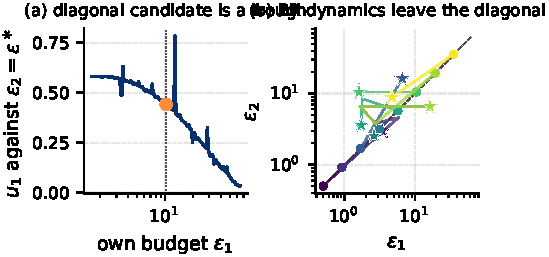
\includegraphics[width=\linewidth]{figures/fig_symmetry_breaking.pdf}
\caption{\textbf{Anatomy of symmetry breaking} ($K=200$ mechanism
cache, symmetric two-player game). \emph{(a)} Player 1's utility
against an opponent fixed at the diagonal first-order candidate
$\eps^\ast$: the symmetric profile (dot) is a local minimum of their
own utility---deviating in either direction pays. \emph{(b)}
Alternating best-response dynamics started at diagonal profiles
(circles): every trajectory leaves the diagonal at the first response
and terminates at an off-diagonal pure Nash equilibrium (stars).}
\label{fig:symbreak}
\end{figure}

\emph{Diagonal trough and the saturation window.} Outside the
saturation window, every feasible diagonal cell admits a strictly
profitable unilateral deviation, with median best-deviation gain
$0.122$ utility across the $200$ diagonal cells
(\cref{fig:symbreak}(a)). The discrete own-action first-order
condition changes sign at eight interior diagonal cells, $\eps^\ast
\in [1.78, 4.07]$; at the lower candidates the trough holds (e.g.\
$\eps^\ast = 2.11$: $+0.007$ upward, $+0.0003$ downward), and at
$\eps^\ast = 2.96$ it flips---both deviations lose, the cell is the
symmetric pure equilibrium of \cref{sec:no-symmetric-ne}.

\emph{Strategic substitutes.} The discrete cross-difference
$u_1(\eps^{+h}_1,\eps^{+h}_2) - u_1(\eps^{+h}_1,\eps^{-h}_2) -
u_1(\eps^{-h}_1,\eps^{+h}_2) + u_1(\eps^{-h}_1,\eps^{-h}_2)$ centred
on diagonal cells is negative on $81.2\%$ / $90.2\%$ / $95.2\%$ of
cells at strides $h = 4$ / $8$ / $16$; the coarser strides average
over the \ac{PLD}-accountant's discreteness and carry the signal.

\emph{Best-response dynamics.} Alternating best-response dynamics
started at each of the $200$ feasible diagonal profiles end
off-diagonal in $197$ cases---the three exceptions start inside the
saturation window and stay at the symmetric equilibrium---with a
median of two steps of play; $134$ of the $200$ runs terminate at a
pure Nash equilibrium within the iteration budget, the remainder in
best-response cycles between near-tied asymmetric profiles
(\cref{fig:symbreak}(b)).

\emph{Symmetric equilibria of the restriction.} Restricted to the
two budgets of the mirror pair $(1.12, 7.13)$, the game is
Hawk--Dove: $u(\textrm{tight}, \textrm{loose}) = (0.505, 0.253)$,
both symmetric profiles of the restriction unstable, and the
restriction's unique symmetric equilibrium mixed, playing tight
with probability $0.445$ at value $0.349$---strictly between the
two role payoffs. On the full $K = 22$ game, exact support
enumeration finds no proper mixed symmetric equilibrium up to
support size five; the game's symmetric equilibrium is the pure one
of the saturation window, present already at that resolution.

\subsection{Proof of \texorpdfstring{\cref{prop:self-sorting}}{the self-sorting proposition}}
\label{app:proof-self-sorting}

Write $f(x, y)$ for player $i$'s realised advantage at own budget $x$
and opponent budget $y$; by $|G_1| = |G_2|$
the noise satisfies $\sigma(x,y) = \sigma(y,x)$ and $f$ is common to
both players. The exchange condition referenced in the main text is
\begin{enumerate}
  \item[\textup{(S)}] for every $x > y$ in the feasible region,
        $\bigl[V(\sigma_H) - V(\sigma_M)\bigr]\,
         \bigl[f(x, y) - f(y, y)\bigr]
         \;\ge\;
         \bigl[V(\sigma_M) - V(\sigma_L)\bigr]\,
         \bigl[f(x, x) - f(y, x)\bigr]$,
\end{enumerate}
where $\sigma_L = \sigma(y,y) > \sigma_M = \sigma(x,y) > \sigma_H =
\sigma(x,x)$ by \cref{lem:externality}.

Fix a pure \ac{NE} interior to the feasible region and suppose for
contradiction $\eps_1^\star > \eps_2^\star$; write $x = \eps_1^\star$,
$y = \eps_2^\star$. With $V' < 0$, both $\Delta V_H := V(\sigma_H) -
V(\sigma_M)$ and $\Delta V_L := V(\sigma_M) - V(\sigma_L)$ are
strictly positive, and by own-budget monotonicity the lifts $D_1 :=
f(x,y) - f(y,y)$ and $D_2 := f(x,x) - f(y,x)$ are strictly positive.
Player 1 not deviating from $x$ to $y$ gives $\lambda_1 D_1 \le \Delta
V_L$; player 2 not deviating from $y$ to $x$ gives $\lambda_2 D_2 \ge
\Delta V_H$. Dividing,
\[
\frac{\lambda_2}{\lambda_1} \;\ge\; \frac{\Delta V_H}{\Delta V_L}\cdot\frac{D_1}{D_2}
\;\ge\; 1
\]
by (S), contradicting $\lambda_1 > \lambda_2$. \qed

Sufficient sub-conditions for (S): $V$ midpoint-convex on
$[\sigma_H, \sigma_L]$ together with $f$ submodular on the
$\{y,x\}^2$ block (which closes in the high-noise regime $\sigma >
\sqrt 3$ via \eqref{eq:sigma-implicit}); or pointwise numerical
verification at the equilibrium candidate, which is how the
$K = 200$ sweeps of \cref{sec:experiments} are certified. At $\lambda_1 =
\lambda_2$, (S) holds with equality and the argument degenerates to
closure of the \ac{NE} set under the swap $(\eps_1,\eps_2)
\leftrightarrow (\eps_2,\eps_1)$---the mirror pairs of
\cref{sec:no-symmetric-ne}.

\subsection{Proof sketch of \texorpdfstring{\cref{thm:continuous-ne-smallp}}{the existence theorem}}

Expand $\partial^2 u_i / (\partial \eps_i \partial \eps_j)$ by the
chain rule. For the shared-$V$ contribution, use the aggregate form
\eqref{eq:sigma-implicit}: writing $S$ for the weighted budget
aggregate, $\sigma_i \sigma_j = \sigma^2 S_i S_j / S^2$ and
$\sigma_{ij} = 2\sigma S_i S_j / S^2$, so
\[
V''(\sigma)\,\sigma_i\sigma_j + V'(\sigma)\,\sigma_{ij}
\;=\; \sigma_i\sigma_j\Bigl[V''(\sigma) +
\tfrac{2V'(\sigma)}{\sigma}\Bigr],
\]
which is $\leq 0$ exactly when $V'' + 2V'/\sigma \leq 0$---for the
canonical $V = 1/(1+\sigma^2)$, when $\sigma \leq \sqrt 3$. The
$-\lambda_i \Apld{i}$ contribution's dominant terms in the small-$p$ regime are
$-\lambda_i A_{i,p\sigma}\,(p_{i,i}\sigma_j + p_{i,j}\sigma_i)$ with
$A_{i,p\sigma} = I\Adv_G'(\sigma) + O(I^2 p_i) < 0$
(\cref{cor:externality-small-p}), and carry the sign of the strictly
negative bracket of \eqref{eq:proof-bracket}. Hence $\partial^2 u_i /
(\partial \eps_i \partial \eps_j) \leq 0$ on the box $\mathcal{B}$: the budgets
are strategic substitutes. For two players, reversing one player's
coordinate turns decreasing differences into increasing differences,
and a box is a compact lattice under any coordinatewise order, so
Milgrom--Roberts (\cite{milgrom1990rationalizability}, Thm.~5)
delivers a non-empty complete lattice of pure \acp{NE} of the
box-restricted game with extremal elements; equilibria of the
restriction whose unrestricted best responses stay inside $\mathcal{B}$ are
equilibria of the \ac{PEG}. The one-coordinate flip is unavailable for $n
> 2$ (substitutes cannot become complements for all pairs at once),
which is why the theorem is stated for two players. Roughly a quarter
of interior cells of the \emph{full} feasible region fail the
numerically tested substitutes sign, so the box qualifier is
not removable with this proof strategy. \qed

\subsection{Proof sketch of \texorpdfstring{\cref{prop:non-potential}}{the non-potential proposition}}

The obstruction is that the externality enters each utility weighted
by the player's own $\lambda_i$ and the \emph{partner's} group size; a
potential would require these weights to reconcile symmetrically
across every pair, which the coupling forbids.

\emph{Cardinal potentials.} Implicit differentiation of
\eqref{eq:sigma-implicit} gives $\sigma_{ij} =
2\sigma\,|G_i||G_j|(r')^2/(rN)^2$ at a symmetric-budget reference,
where $r := \sqrt{\rho}$ and $N := \sum_g|G_g|$; the shared-$V$
contribution to the Monderer--Shapley cross-partial condition
$\eta_j\, \partial^2 u_i / \partial\eps_i\partial\eps_j = \eta_i\,
\partial^2 u_j / \partial\eps_i\partial\eps_j$ is symmetric under
$i\leftrightarrow j$ and cancels. Expanding the $\Apld{i}$ contribution
reduces the residual to $\eta_j \lambda_i |G_j|(2|G_i| - N) = \eta_i \lambda_j
|G_i|(2|G_j| - N)$ at every symmetric profile, which has no positive
solution $(\eta_i,\eta_j)$ for $|G_i| \neq |G_j|$; in the fully
symmetric case the residual carries $(\eta_j - \eta_i)\,d^2 V$, which
is nonconstant along the feasible interval and cannot vanish
uniformly unless $\eta_1 = \eta_2$, in which case the heterogeneous
case above bites.

\emph{Ordinal potentials.} By \cite{monderer1996potential},
Lemma~2.5, an ordinal potential precludes strict improvement cycles.
On the $K=22$ discretisation of the canonical game, the cycle
$(1.587,5.040) \to (2.000,5.040) \to (2.000,4.000) \to (1.587,4.000)
\to (1.587,5.040)$ has each step strictly improving for the deviating
player (unilateral gains $7.3\times 10^{-7}$, $1.5\times 10^{-3}$,
$3.0\times 10^{-3}$, $2.8\times 10^{-3}$, re-verified from the
mechanism cache). One caveat for the record: the smallest of the four
gains sits near the accountant's numerical resolution; the cycle's
existence does not hinge on it alone---three of the four steps exceed
$10^{-3}$---but a fully tolerance-robust cycle would re-solve the
four profiles at finer \ac{PLD} discretisation. \qed

\section{Validity and role of \texorpdfstring{$V$}{V}}
\label{app:V}

\citet{bassily2014private} prove that for a $1$-Lipschitz
strongly-convex loss, the excess empirical risk of DP-ERM satisfies
$\E[\hat L(\widehat\theta) - \hat L(\theta^*)] =
O\!\left(d\log(1/\delta)/(n^2\eps^2)\right)$; under the moments
accountant of \citet{abadi2016deep} this translates into a $\sigma^2
d/n^2$ dependence. Treating model utility as the negative of excess
risk and renormalising to $[0,1]$ gives $V(\sigma) \propto
1/(1+\alpha\sigma^2)$ for a problem constant $\alpha$; we set
$\alpha=1$. The bound assumes convexity; the empirical \ac{DPSGD}
literature~\cite{tramer2021private, abadi2016deep, boenisch2023have}
confirms the same qualitative direction in deep learning. The
following pair, referenced from \cref{sec:analysis}, confines $V$'s
analytical role to $\mathrm{sgn}\,V'$.

\begin{assumption}[Admissible model-utility function]
\label[assumption]{ass:V-admissible}
$V\colon \sigma(\mathcal F) \to \R$ is \emph{admissible} iff it is
continuous, strictly decreasing, and bounded on the feasible noise
range.
\end{assumption}

\begin{proposition}[Qualitative invariance in $V$]
\label[proposition]{prop:V-invariance}
For every admissible $V$: (i) the externality signs of
\cref{lem:externality,cor:externality-small-p,prop:externality-full}
hold; (ii) \cref{cor:coalition-attack} holds; and (iii) at any
interior best response, \eqref{eq:foc} depends on $V$ only through
$\mathrm{sgn}\,V'$.
\end{proposition}

The proof is by
inspection: the mechanism constraints \eqref{eq:budget}--\eqref{eq:batch} and the closed form
$p_g(\sigma,\eps_g)$ never read $V$, so
\cref{lem:externality,cor:externality-small-p,prop:externality-full}
and \cref{cor:coalition-attack} (which uses only the externality sign
on the target's coordinate) are $V$-free; differentiating
\eqref{eq:utility} in $\eps_i$ gives \eqref{eq:foc}, whose sign
structure reads $V$ only through $\mathrm{sgn}\,V'$; and continuity
plus boundedness make the discretised game well-defined for every
admissible $V$.

\subsection{Numerical ablation over admissible shapes}
\label{app:v-shape}

We re-enumerate the canonical $K = 200$ equilibria under six
admissible shapes: the canonical $V_1(\sigma) = 1/(1+\sigma^2)$, the
slow-decaying $V_2 = 1/(1+\sigma)$, the Gaussian $V_3 =
e^{-\sigma^2/2}$, the exponential $V_4 = e^{-\sigma}$, the concave
$V_5 = -\log(1+\sigma)$, and the affine $V_6 = -\sigma$. Because the
mechanism grid is $V$-free, each shape costs only $O(K^2)$
elementwise work on the cached tensor.

\begin{figure}[t]
  \centering
  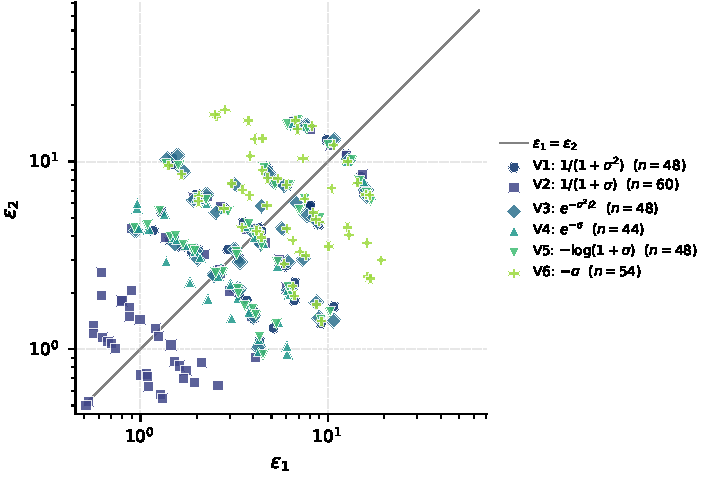
\includegraphics[width=0.9\linewidth]{figures/fig_h5_v_shape.pdf}
  \caption{\textbf{Model-utility ablation} ($K=200$, $\lambda=1$). Pure \ac{NE}
    locations under six admissible shapes for $V$. Under every shape,
    $100\%$ of the pure \acp{NE} sit off the diagonal.}
  \label{fig:H5-v-shape}
\end{figure}

\begin{table}[t]
  \centering
  \small
  \begin{tabular}{l l r r r}
    \toprule
    tag & shape & \#\ac{NE} & $\mathrm{mean}(b\!\to\!a)$ & agree$_{\mathrm{sign}}$ \\
    \midrule
    $V_1$ & $1/(1+\sigma^2)$   & 48 & 0.000 & 100.0\% \\
    $V_2$ & $1/(1+\sigma)$     & 60 & 0.075 & 100.0\% \\
    $V_3$ & $e^{-\sigma^2/2}$  & 48 & 0.013 & 100.0\% \\
    $V_4$ & $e^{-\sigma}$      & 44 & 0.062 & 100.0\% \\
    $V_5$ & $-\log(1+\sigma)$  & 48 & 0.000 & 100.0\% \\
    $V_6$ & $-\sigma$          & 54 & 0.111 & 100.0\% \\
    \bottomrule
  \end{tabular}
  \caption{Per-$V$ pure-\ac{NE} count, mean one-sided Hausdorff distance
    from a $V_1$-\ac{NE} to its nearest \ac{NE} under $V_k$ (decades of
    $\log_{10}\eps$), and externality-sign agreement with $V_1$ over
    interior feasible edges. $K = 200$, $\lambda = 1$.}
  \label{tab:H5-v-shape}
\end{table}

Across the six shapes the pure-\ac{NE} count stays in $44$--$60$ and the
\ac{NE} set remains entirely off-diagonal (\cref{fig:H5-v-shape},
\cref{tab:H5-v-shape}); each $V_1$-equilibrium has a match within
$0.11$ decades under every alternative; and the externality-sign
pattern over feasible edges agrees with $V_1$ on $100\%$ of edges---
the numerical fingerprint of the additive separation of
\eqref{eq:utility}, in which the sign of $\partial u_i / \partial
\eps_j$ is mechanism-determined and $V$-free.

\section{The externality response and its sign certificate}
\label{app:certificate}

\paragraph{The externality in isolation.} The equilibrium results all
flow through one primitive: the response of a target's realised
advantage to the others' budgets. We isolate it by fixing the
target's budget $\eps_T \in \{4, 16\}$ and sweeping the other group's
budget $\eps_O$ and dataset share (\cref{fig:C5}). The dependence is
smooth and monotone, exactly as \cref{prop:externality-full} predicts:
at $\eps_T = 4$ the target's advantage runs from $0.20$ (others at
$\eps_O = 0.5$) to near zero (others at $64$); at $\eps_T = 16$, from
$0.55$ down to $0.05$. The curves for different shares cross at
$\eps_O = \eps_T$, where the others' contribution to $\sigma$ matches
the target's own; below the crossover a larger foreign share
amplifies the externality, above it, suppresses it.

\begin{figure*}[!t]
\centering
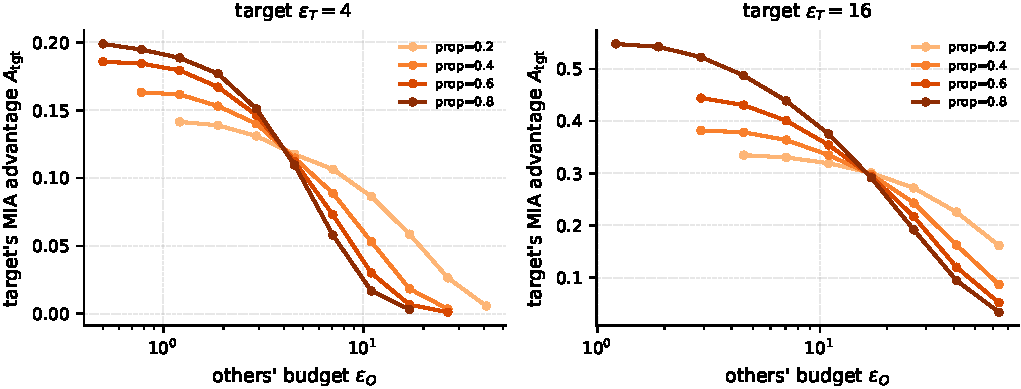
\includegraphics[width=\linewidth]{figures/fig_C5_surface.pdf}
\caption{\textbf{The externality in isolation.} Target's realised \ac{MIA}
advantage as a function of the other group's budget $\eps_O$ and
dataset share, at fixed target budgets $\eps_T \in \{4, 16\}$. The
dependence is monotone in $\eps_O$; curves cross at $\eps_O =
\eps_T$, with larger foreign shares amplifying the externality below
the crossover and suppressing it above.}
\label{fig:C5}
\end{figure*}

\paragraph{Finite-difference certificate.}
This is the certificate that part (ii) of
\cref{prop:externality-full} relies on beyond the small-$p$ regime
(\cref{app:proof-full-region}): we certify the sign on the $K=200$
mechanism cache by finite differences. Of the $40{,}000$ grid
cells, $64.5\%$ are feasible, matching the analytic participation
frontier cell-for-cell. At unit stride---one grid step, no
smoothing---the predicted cross-sign $\partial \Apld{i}/\partial
\eps_j < 0$ holds at every one of the $25{,}612$ feasible interior
differences, and the own-direction sign $\partial \Apld{i}/\partial
\eps_i > 0$ likewise at $25{,}612$ of $25{,}612$. The certificate
is exhaustive on the feasible region; no stride averaging or
jitter exclusion is required.

\section{Symmetric weight sweep}
\label{app:wsweep}

Sweeping the \emph{common} weight $\lambda \in \{0.125, 0.25, 0.5, 1, 2,
4\}$ for both players moves how much everyone cares, without breaking
symmetry (\cref{fig:C7}). On the utility-leaning half of the sweep
the asymmetric structure is insensitive: $\lambda \in \{0.125, 0.25,
0.5\}$ yields $34$--$62$ pure \acp{NE}, all off-diagonal, and
$\lambda = 1$ adds the saturation-window equilibrium to its $42$
asymmetric ones. The privacy-heavy extreme is different in kind: at
$\lambda = 2$ the grid has \emph{no} pure equilibrium---only mixed
play survives---and at $\lambda = 4$ a single corner equilibrium
$(0.5, 0.5)$ remains. The weight also moves \emph{where} the cloud
sits (privacy-heavy play compresses budgets downward) and how
costly equilibrium play is in aggregate, quantified in
\cref{sec:poev}: at $\lambda \le 0.25$ \emph{every} equilibrium
inflates aggregate advantage over the uniform baseline (up to
$+165\%$), at $\lambda = 0.5$ still $94\%$ of them do, while at
$\lambda = 1$ only $14\%$ do and the $\lambda = 4$ corner deflates
it by $82\%$.

\begin{figure}[!t]
\centering
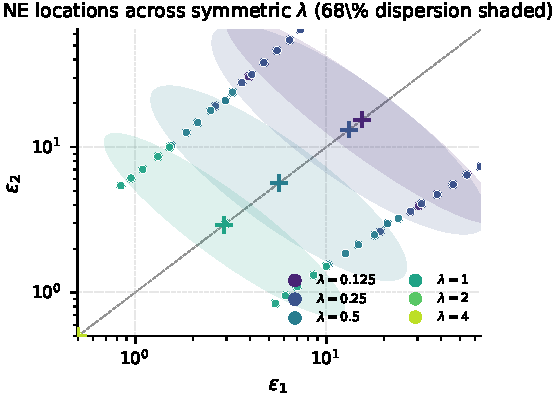
\includegraphics[width=\linewidth]{figures/fig_C7_lambda_ratio.pdf}
\caption{\textbf{Symmetric weight sweep} ($K=200$). Pure \ac{NE} clouds at
common weights $\lambda \in \{0.125, \dots, 4\}$ (centroids and $68\%$
dispersion ellipses); the dashed line is the diagonal. The \ac{NE}
set stays off-diagonal at every weight except the $\lambda = 1$
saturation-window equilibrium and the $\lambda = 4$ corner $(0.5,
0.5)$; at $\lambda = 2$ no pure equilibrium exists. The cloud shifts
toward lower budgets as privacy weight grows.}
\label{fig:C7}
\end{figure}

\section{The Bayesian Repeated PEG in full}
\label{app:bayesian}

\paragraph{Position in the literature.} The classical framework for
repeated play under one-sided private information is
\citet{aumann1995repeated}, whose central question is how the
informed player manages what they reveal. The security-motivated
strand has a leader committing each round against a follower of
unknown type, refining a belief over the follower's payoff from
observed responses~\cite{letchford2009learning, blum2014learning,
balcan2015commitment}; \citet{kalai1993rational} supply the
posterior-consistency backbone. Selling privacy at heterogeneous
private valuations~\cite{ghosh2011selling} and Bayesian
persuasion~\cite{kamenica2011bayesian} are conceptually adjacent but
solve different design problems. The BR-PEG of \cref{sec:brpeg} is
the Stackelberg-learning template with the tabular follower payoff
replaced by the DP-accountant coupling of \cref{def:sampling-idp};
the follower's private type is $\theta_H = (\lambda_H, n_H)$, the leader
observes $(\eps_H^t, u_H^t)$ after each round, and the finite type
space with a full-support prior makes Kalai--Lehrer merging
automatic---the interesting content is what the leader does once the
posterior concentrates.

\paragraph{Full proof of \cref{prop:bayesian-not-min}.} Write $\bar
G(\eps_M; \pi) := \mathbb{E}_{\theta \sim \pi} G(\eps_M; \theta)$
for the posterior-averaged score, a finite mixture of per-type
scores, continuous in $\pi$ in total variation and defined on the
finite grid $\mathcal{A}$.

\emph{Step 1 (posterior collapse).} By identifiability (I) and
\citet{kalai1993rational}, $\pi^t \to \delta_{\theta_H^\star}$
$\pi^0$-a.s.: any type producing a distinct best response at the
leader's action contributes strictly positive KL divergence per
round, and divergences accumulate.

\emph{Step 2 (uniform score convergence).} $G$ is bounded in $[0,1]$,
so for every arm, $|\bar G(\eps_M; \pi^t) - G(\eps_M;
\theta_H^\star)| \leq 1 - \pi^t(\theta_H^\star) \to 0$, uniformly
over the finite $\mathcal{A}$.

\emph{Step 3 (argmax lock-in).} Let $\gamma > 0$ be the truth-argmax
gap from (A) (not to be confused with the contract parameter
$\Delta$). Once $1 - \pi^t(\theta_H^\star) < \gamma/2$, for any
$\eps_M \neq \eps_M^\star$,
\[
\bar G(\eps_M^\star; \pi^t) - \bar G(\eps_M; \pi^t)
\;\geq\; \gamma - 2\bigl(1 - \pi^t(\theta_H^\star)\bigr) \;>\; 0,
\]
so the posterior-greedy arm equals $\eps_M^\star$ for all subsequent
rounds; separation from $\eps^{\min}$ is (A). \qed

\paragraph{Clean demo instance.} With three well-separated types
($\Theta = \{\lambda_H \in \{0.5, 1, 2\}\}$, truth $\lambda_H^\star = 2$, $n_H =
n_M = 5000$, canonical parameters), the posterior collapses after a
single round; from $t = 1$ the Bayesian-greedy leader plays
$\eps_M^\star \approx 3.08$, eliciting $\eps_H \approx 19$ and $A_H
\approx 0.454$ per round---roughly $2\times$ the naive constant
attack $\eps_M = 1$ ($A_H \approx 0.22$) and $\approx 50\times$ the
benign baseline $\eps_M = 64$ ($A_H \approx 0.01$)
(\cref{fig:bayesian}). Assumption (A) is verified on the mechanism
grid: the argmax is interior ($\approx 2.1$ above the naive
anchor), because the leader's gain comes from eliciting a more
exposing best response, not from forcing $\sigma$ down. The regret
instance of \cref{fig:regret} hardens this demo---five overlapping
types whose best responses coincide at several arms and observation
noise $\sigma_{\mathrm{obs}} = 0.15$ on $u_H$---so that
identification takes $\approx 10$ rounds rather than one and the
regret separation between correct-prior, misspecified-prior, and
prior-free attackers becomes visible.

\begin{figure*}[!t]
\centering
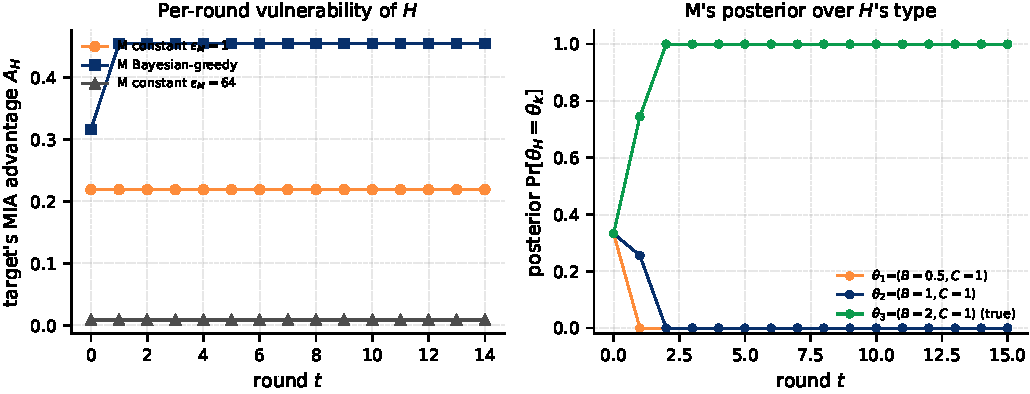
\includegraphics[width=0.95\linewidth]{figures/fig_bayesian.pdf}
\caption{\textbf{BR-PEG demo} (three well-separated types). Left:
per-round realised advantage $A_H$ under three leader policies.
Right: the leader's posterior over $\theta_H$ under the
Bayesian-greedy policy; it collapses to the truth within one round.}
\label{fig:bayesian}
\end{figure*}

\paragraph{What remains open.} A strategising target---one who
manages what their responses reveal, the two-sided game of
\citet{aumann1995repeated}---and finite-horizon regret rates in the
style of \citet{balcan2015commitment, blum2014learning} both fit the
framework without modification and are left open.

\section{Non-strategyproofness and the type-channel design problem}
\label{app:mechanism-design}

\paragraph{Environment.} Player $i$'s group size is public; their type
is their privacy weight $\lambda_i > 0$, private. A direct-revelation \ac{iDP}
mechanism maps reported budgets to a mechanism solution satisfying
\eqref{eq:budget}--\eqref{eq:batch}, with no transfers; sampling-based \ac{iDP} as deployed is the
\emph{identity mechanism} on the budget channel.

\paragraph{Proof of \cref{prop:non-strategyproof}.} Fix $i$ and $\lambda_i
> 0$. Choose opponent profiles on opposite sides of the externality:
$\hat{\boldsymbol{\eps}}_{-i}^{\mathrm{L}}$ loose, $\hat{\boldsymbol{\eps}}_{-i}^{\mathrm{T}}$
tight. By \cref{lem:externality} and the certified sign of
\cref{prop:externality-full},
pointwise on $\Sigma_i$: $\sigma^{\mathrm{T}} > \sigma^{\mathrm{L}}$ and $\Apld{i}^{\mathrm{T}} \geq
\Apld{i}^{\mathrm{L}}$, and the marginal utilities $\partial_{\hat\eps_i} u_i^{K} =
V'(\sigma^{K})\partial_{\hat\eps_i}\sigma^{K} - \lambda_i
\partial_{\hat\eps_i} \Apld{i}^{K}$ differ across $K \in \{\mathrm{L}, \mathrm{T}\}$, so the
best-response maps differ. A numerical witness in a scaled two-player
instance ($|G_1|=|G_2|=25{,}000$, $B=128$, $I=1953$,
$\delta=10^{-12}$, $\lambda_1=1$):
against $\hat\eps_2 = 4.0$ the best report is $\hat\eps_1 \approx
2.92$; against $\hat\eps_2 = 0.5$ it is $\approx 1.21$. Sweeping
$\hat\eps_2$ over the grid, the best-response report takes six
distinct values, generally rising with $\hat\eps_2$. No single report
dominates. \qed

\paragraph{Why the classical escapes fail.} The large-market recovery
of~\cite{kearns2014mechanism} requires single-agent influence to
vanish; a silo moves \eqref{eq:batch} at $\Theta(1)$. The impossibility results
for unbounded privacy valuations~\cite{nissim2014redrawing,
ghosh2011selling} are not the obstacle (utility here is bounded); the
obstacle is the coupled $\sigma$: the positive results
of~\cite{chen2013truthful} model privacy costs that vanish when a
report has no influence on the outcome, whereas in the \ac{PEG} every
report moves $\sigma$.

\paragraph{The type-channel problem.} A repair would elicit $\lambda_i$
rather than $\eps_i$ and allocate budgets centrally. With transfers,
the envelope route reduces Bayesian incentive compatibility to
monotonicity of the interim advantage $\overline{A}_i(\lambda_i)$ in the
reported type~\cite{myerson1981optimal, rochet1987necessary,
roberts1979characterization}; three features keep the full theorem
open here: the mechanism must choose one shared $\sigma$; the interim
advantage couples all opponents' types through the joint solve; and
there is no monetary transfer, leaving excess realised vulnerability
as the only in-kind instrument---itself the quantity the contract
constrains. We leave the constructive design problem to future work.

\section{Sensitivity checks}
\label{app:sensitivity}

Grid refinement from $K=22$ through $K=200$ multiplies the resolved
pure-\ac{NE} count ($8 \to 48$) while preserving the structural
invariants---zero diagonal equilibria, mirror pairing, the
budget-ratio band, and the BR-loci geometry (\cref{sec:no-symmetric-ne}).
Substituting admissible alternatives for $V$ preserves the structure
(\cref{app:v-shape}). On a $K' = 50$ subgrid of the canonical game,
the equilibrium count is insensitive to \emph{lowering} the
participation threshold ($12$ pure \acp{NE} at both $10^{-5}$ and
$10^{-7}$, over identical feasible regions) and drops to $6$ only
when the threshold is raised to $10^{-3}$, which prunes boundary
equilibria while leaving interior equilibria and all reported signs
unchanged; the externality-sign certificate improves slightly under
the stricter threshold ($95.5\%$ at $10^{-3}$ versus $92.7\%$ at
$10^{-5}$ at matched stride). Sweeps over $\delta$, batch size and
epoch count, and the accountant's R\'enyi orders are deferred to
follow-up runs.
